\begin{name}
{Đề Ôn Tập HS TB-Yếu}
{Năm học 2025-2026}
\end{name}

\Opensolutionfile{ans}[ans/De-TB-Yeu-So-19]
\cautn
\begin{ex}%[1D2N2-2]
	Dãy số nào sau đây là một cấp số cộng?
	\choice
	{$1$; $5$; $7$; $8$; $\dots$}
	{$2$; $3$; $6$; $7$; $10$; $\dots$}
	{\True $6$; $8$; $10$; $12$; $14$; $\dots$}
	{$5$; $8$; $4$; $12$; $\dots$}
	\loigiai{
		Dãy số $6$; $8$; $10$; $12$; $14$; $\dots$ có hiệu của hai số hạng liên tiếp luôn bằng $2$ (không đổi) nên nó là cấp số cộng.
	}
\end{ex}

\begin{ex}%[2D1H4-1]
	Cho hàm số $y=f(x)$ xác định, liên tục trên $\mathbb{R}\setminus\{1\}$ và có bảng biến thiên ở hình vẽ.
	\begin{center}
	
\begin{tikzpicture}
		\tkzTabInit[nocadre=false, lgt=1.2, espcl=2.5, deltacl=0.6]{$x$/0.6,$y'$/0.6,$y$/2}
		{$-\infty$, $-1$, $0$, $1$, $+\infty$}
		\tkzTabLine {,+,0,-,0,+,d,-,}
		\tkzTabVar{-/ $-\infty$, +/ $1$, -/$0$, +D+ / $+\infty$ / $+\infty$, -/ $-\infty$}
	\end{tikzpicture}
	\end{center}
	Tổng số tiệm cận đứng và tiệm cận ngang của đồ thị hàm số đã cho là
	\choice
	{$0$}
	{$3$}
	{$2$}
	{\True $1$}
	\loigiai{
		Từ bảng biến thiên ta thấy
\begin{itemize}
\item $\lim \limits_{x\to -\infty}f(x)=-\infty$ và $\lim \limits_{x\to +\infty}f(x)=+\infty$, suy ra đồ thị hàm số không có tiệm cận ngang. 
\item $\lim \limits_{x\to 1^-}f(x)=-\infty$ và $\lim \limits_{x\to 1^+}f(x)=+\infty$, suy ra đồ thị hàm số có $1$ tiệm cận đứng là đường thẳng $x=1$. 
\end{itemize}
		Vậy tổng số tiệm cận đứng và tiệm cận ngang của đồ thị hàm số đã cho là $1$.
	}
\end{ex}

\begin{ex}%[2D5H1-2]
	Cho hai biến cố độc lập $A$, $B$ với $\mathrm{P}(A)=0{,}8$, $\mathrm{P}(B)=0{,}3$. Khi đó, $\mathrm{P}(A|B)$ bằng
	\choice
	{$0{,}6$}
	{$0{,}3$}
	{$0{,}4$}
	{\True $0{,}8$}
	\loigiai{
		Do $A,B$ là hai biến cố độc lập nên $\mathrm{P}(A\cap B)=\mathrm{P}(A)\cdot \mathrm{P}(B)$. \\
		Áp dụng công thức xác suất có điều kiện 
		$\mathrm{P}(A|B)=\dfrac{\mathrm{P}(A\cap B)}{\mathrm{P}(B)}=\dfrac{\mathrm{P}(A)\cdot \mathrm{P}(B)}{\mathrm{P}(B)}=\mathrm{P}(A)=0{,}8$.
	}
\end{ex}

\begin{ex}%[2H5N3-3]
	Trong không gian $Oxyz$, phương trình mặt cầu có tâm $I(1;-2;3)$ bán kính $R=2$ là
	\choice
	{$(x-1)^2+(y+2)^2+(z-3)^2=2$}
	{$(x+1)^2+(y-2)^2+(z+3)^2=4$}
	{$(x+1)^2+(y-2)^2+(z+3)^2=2$}
	{\True $(x-1)^2+(y+2)^2+(z-3)^2=4$}
	\loigiai{
		Phương trình mặt cầu có tâm $I(1;-2;3)$, bán kính $R=2$ là $(x-1)^2+(y+2)^2+(z-3)^2=4$.
	}
\end{ex}

\begin{ex}%[1H8N7-1]
	Cho một hình chóp có đáy là hình vuông cạnh bằng $a$, có thể tích $V$, chiều cao $h$. Khi đó $h$ được xác định bởi công thức nào sau đây?
	\choice
	{$h=\dfrac{V}{a^2}$}
	{$h=\dfrac{V}{3a^2}$}
	{\True $h=\dfrac{3V}{a^2}$}
	{$h=\dfrac{a^2}{3V}$}
	\loigiai{
		Diện tích đáy hình vuông cạnh $a$ là $S=a^2$. \\
		Thể tích khối chóp là $V=\dfrac{1}{3}S\cdot h=\dfrac{1}{3}a^2\cdot h$. \\
		Từ đó suy ra $h=\dfrac{3V}{a^2}$.
	}
\end{ex}

\begin{ex}%[1D5N1-1]
	Giá trị đại diện của nhóm $[a_i;a_{i+1})$ là
	\choice
	{$\dfrac{a_{i+1}-a_i}{2}$}
	{$\dfrac{a_i+a_{i-1}}{2}$}
	{\True $\dfrac{a_i+a_{i+1}}{2}$}
	{$a_i$}
	\loigiai{
Giá trị đại diện của nhóm $[a_i;a_{i+1})$ là $\dfrac{a_i+a_{i+1}}{2}$.
	}
\end{ex}

\begin{ex}%[1H8N6-1]
	Mệnh đề nào đúng trong các mệnh đề sau?
	\choice
	{Góc giữa đường thẳng $a$ và mặt phẳng $(P)$ bằng góc giữa đường thẳng $b$ và mặt phẳng $(P)$ thì $a$ và $b$ song song}
	{Góc giữa đường thẳng $a$ và mặt phẳng $(P)$ bằng góc giữa đường thẳng $a$ và mặt phẳng $(Q)$ thì mặt phẳng $(P)$ song song với mặt phẳng $(Q)$}
	{\True Góc giữa đường thẳng và mặt phẳng bằng góc giữa đường thẳng đó và hình chiếu của nó trên mặt phẳng đã cho}
	{Góc giữa đường thẳng $a$ và mặt phẳng $(P)$ bằng góc giữa đường thẳng $b$ và mặt phẳng $(P)$ khi $a$ và $b$ song song}
	\loigiai{
		Theo định nghĩa góc giữa đường thẳng và mặt phẳng trong không gian: Nếu đường thẳng không vuông góc với mặt phẳng, góc giữa đường thẳng và mặt phẳng là góc giữa đường thẳng đó và hình chiếu vuông góc của nó trên mặt phẳng đã cho.
	}
\end{ex}

\begin{ex}%[2D4H1-2]
	Họ nguyên hàm của hàm số $f(x)=\dfrac{1}{x^2}-x^2-\dfrac{1}{3}$ là
	\choice
	{$-\dfrac{x^4+x^2+3}{3x}+C$}
	{$-\dfrac{2}{x^2}-2x+C$}
	{\True $\dfrac{-x^3}{3}-\dfrac{1}{x}-\dfrac{x}{3}+C$}
	{$\dfrac{-x^4+x^2+3}{3x}+C$}
	\loigiai{
		Ta có $\displaystyle\int \left(\dfrac{1}{x^2}-x^2-\dfrac{1}{3}\right)\,\mathrm{d}x=\displaystyle\int \left(x^{-2}-x^2-\dfrac{1}{3}\right)\,\mathrm{d}x=\dfrac{x^{-1}}{-1}-\dfrac{x^3}{3}-\dfrac{1}{3}x+C=-\dfrac{1}{x}-\dfrac{x^3}{3}-\dfrac{x}{3}+C$.
	}
\end{ex}

\begin{ex}%[1D6N4-2]
	Phương trình $2023^x=1$ có nghiệm là:
	\choice
	{$x=2023$}
	{$x=1$}
	{\True $x=0$}
	{$x=-1$}
	\loigiai{
		Ta có $2023^x=1\Leftrightarrow 2023^x=2023^0\Leftrightarrow x=0$.
	}
\end{ex}

\begin{ex}%[2H5N1-5]
	Trong không gian $Oxyz$, khoảng cách từ điểm $A(0;0;5)$ đến mặt phẳng $(P)\colon x+2y+2z-3=0$ bằng
	\choice
	{$\dfrac{8}{3}$}
	{\True $\dfrac{7}{3}$}
	{$\dfrac{4}{3}$}
	{$3$}
	\loigiai{
Ta có $\mathrm{d}(A,(P))=\dfrac{|0+2\cdot 0+2\cdot 5-3|}{\sqrt{1^2+2^2+2^2}}=\dfrac{7}{\sqrt{9}}=\dfrac{7}{3}$.
	}
\end{ex}

\begin{ex}%[2D1N2-2]
	Cho hàm số $y=f(x)$ có bảng biến thiên như sau:
	\begin{center}
	
\begin{tikzpicture}
		\tkzTabInit[nocadre=false, lgt=1.2, espcl=2.5, deltacl=0.6]{$x$/0.6,$y'$/0.6,$y$/2}
		{$-\infty$, $-1$, $2$, $+\infty$}
		\tkzTabLine {,+,0,-,0,+,}
		\tkzTabVar{-/ $-\infty$, +/ $5$, -/ $-6$, +/ $+\infty$}
	\end{tikzpicture}
	\end{center}
	Mệnh đề nào dưới đây đúng?
	\choice
	{Hàm số có $4$ điểm cực trị}
	{Hàm số không có cực đại}
	{Hàm số đạt cực tiểu tại $x=-6$}
	{\True Hàm số đạt cực tiểu tại $x=2$}
	\loigiai{
Bảng biến thiên cho thấy hàm số đã cho đạt cực tiểu tại $x=2$.
	}
\end{ex}

\begin{ex}%[1D6H2-2]
	Cho $a=\log _25$, $b=\log _29$. Biểu diễn của $P=\log _2\dfrac{40}{3}$ theo $a$ và $b$ là
	\choice
	{$P=3+a-2b$}
	{$P=3+a-\sqrt{b}$}
	{\True $P=3+a-\dfrac{1}{2}b$}
	{$P=\dfrac{3a}{2b}$}
	\loigiai{
		Ta có \begin{itemize}
\item $P=\log _2\dfrac{40}{3}=\log _240-\log _23$,
\item $\log _240=\log _2(8\cdot 5)=\log _28+\log _25=3+a$,
\item $b=\log _29=\log _2(3^2)=2\log _23\Rightarrow \log _23=\dfrac{1}{2}b$. 
\end{itemize}
Vậy $P=3+a-\dfrac{1}{2}b$.
	}
\end{ex}

\cauds
\begin{ex}%[2H5H2-4]
	Trong không gian $Oxyz$, cho đường thẳng $\Delta _1\colon \heva{&x=1+t\\&y=2+3t\\&z=3-t}$ và đường thẳng $\Delta _2\colon \dfrac{x-2}{-2}=\dfrac{y+2}{1}=\dfrac{z-1}{3}$.
	\choiceTF
	{Hai đường thẳng $\Delta _1$ và $\Delta _2$ chéo nhau}
	{$\cos (\Delta _1,\Delta _2)=\dfrac{2\sqrt{154}}{77}$}
	{\True Đường thẳng $d$ đi qua điểm $N(2;3;-1)$ đồng thời cắt và vuông góc với $\Delta _2$ có phương trình là $\dfrac{x-2}{2}=\dfrac{y-3}{-71}=\dfrac{z+1}{25}$}
	{\True Điểm $M(1;2;3)$ thuộc $\Delta _1$ và điểm $N(2;-2;1)$ thuộc $\Delta _2$}
	\loigiai{
		\begin{itemchoice}
			\itemch Đường thẳng $\Delta _1$ có vectơ chỉ phương $\overrightarrow{u}_1=(1;3;-1)$ và đi qua $M(1;2;3)$. \\
			Đường thẳng $\Delta _2$ có vectơ chỉ phương $\overrightarrow{u}_2=(-2;1;3)$ và đi qua $N(2;-2;1)$. \\
			Ta có $\left[\overrightarrow{u}_1,\overrightarrow{u}_2\right]=(10;-1;7)$ và $\overrightarrow{MN}=(1;-4;-2)$. \\
			Ta tính được $\left[\overrightarrow{u}_1,\overrightarrow{u}_2\right]\cdot \overrightarrow{MN}=10\cdot 1+(-1)\cdot (-4)+7\cdot (-2)=10+4-14=0$ nhưng $\overrightarrow{u}_1$ và $\overrightarrow{u}_2$ không cùng phương, nên $\Delta _1$ và $\Delta _2$ cắt nhau.
			\itemch Ta có $\cos (\Delta _1,\Delta _2)=\dfrac{\left|\overrightarrow{u}_1\cdot \overrightarrow{u}_2\right|}{\left|\overrightarrow{u}_1\right|\cdot \left|\overrightarrow{u}_2\right|}=\dfrac{|1\cdot (-2)+3\cdot 1+(-1)\cdot 3|}{\sqrt{1^2+3^2+(-1)^2}\cdot \sqrt{(-2)^2+1^2+3^2}}=\dfrac{\sqrt{154}}{77}\ne\dfrac{2\sqrt{154}}{77}$.
			\itemch Gọi $P=d\cap \Delta _2$. Ta có $P\in \Delta _2\Rightarrow P(-2t+2;t-2;3t+1)$. \\
			Vectơ $\overrightarrow{NP}=(-2t;t-5;3t+2)$. \\
			Vì $d\perp \Delta _2$ nên $\overrightarrow{NP}\cdot \overrightarrow{u}_2=0\Leftrightarrow -2\cdot (-2t)+1\cdot (t-5)+3\cdot (3t+2)=0\Leftrightarrow 14t+1=0\Leftrightarrow t=-\dfrac{1}{14}$. \\
			Suy ra $\overrightarrow{NP}=\left(\dfrac{1}{7};-\dfrac{71}{14};\dfrac{25}{14}\right)$. Chọn vectơ chỉ phương $\overrightarrow{u}_d=14\overrightarrow{NP}=(2;-71;25)$. \\
			Phương trình đường thẳng $d$ là $\dfrac{x-2}{2}=\dfrac{y-3}{-71}=\dfrac{z+1}{25}$.
			\itemch Điểm $M(1;2;3)$ thuộc $\Delta _1$ và điểm $N(2;-2;1)$ thuộc $\Delta _2$.
		\end{itemchoice}
	}
\end{ex}

\begin{ex}%[2D5H1-4]
	Một nhóm học sinh gồm $12$ nam và $13$ nữ đi tham quan Công viên nước Hạ Long, tới lúc tham gia trò chơi mỗi học sinh chọn một trong hai trò chơi là Sóng thần hoặc Đảo hải tặc. Xác suất chọn trò chơi Sóng thần của mỗi học sinh nam là $0{,}6$ và của mỗi học sinh nữ là $0{,}3$. Chọn ngẫu nhiên một bạn của nhóm. Xét tính đúng, sai của mỗi khẳng định sau?
	\choiceTF
	{\True Xác suất để bạn được chọn là nam là $0{,}48$}
	{\True Xác suất để bạn được chọn là nữ và tham gia trò chơi Sóng thần là $0{,}156$}
	{Xác suất để bạn được chọn là nam và tham gia trò chơi Đảo hải tặc là $0{,}195$}
	{Xác suất để bạn được chọn là nữ là $0{,}5$}
	\loigiai{
Gọi \begin{itemize}
\item $A$ là biến cố \lq\lq chọn được bạn nam\rq\rq,
\item $B$ là biến cố \lq\lq chọn được bạn tham gia trò chơi Sóng thần\rq\rq.
\end{itemize}
Theo đề bài ta có, $\mathrm{P}(A)=\dfrac{12}{25}=0{,}48$, $\mathrm{P}\left(\overline{A}\right)=0{,}52$, $\mathrm{P}(B\mid A)=0{,}6$ và $\mathrm{P}\left(B\mid \overline{A}\right)=0{,}3$.\\
Ta có sơ đồ cây như dưới đây
\begin{center}
\begin{tikzpicture}[>=stealth, line join=round, line cap=round, scale=1]
    \coordinate (O) at (0,0);
    \foreach \y/\id/\text/\val/\pos in {
        1.5/Nam/Nam/0{,}48/above left, 
       -1.5/Nu/Nữ/0{,}52/below left%
    } {
        \node (\id) at (3, \y) {\text};
        \draw[->, blue] (O) -- (\id.west) node[pos=0.6, \pos, black] {$\val$};
    }
    \foreach \parent/\y/\id/\text/\val/\pos/\event/\result in {
        Nam/ 2.5/ST1/Sóng thần/0{,}60/above left/AB/0{,}288,
        Nam/ 0.5/DHT1/Đảo hải tặc/0{,}40/below left/A\overline{B}/0{,}192,
        Nu/-0.5/ST2/Sóng thần/0{,}30/above left/\overline{A}B/0{,}156,
        Nu/-2.5/DHT2/Đảo hải tặc/0{,}70/below left/\overline{A}\overline{B}/0{,}364%
    } {
        \node[right] (\id) at (6, \y) {\text};
        \draw[->] (\parent.east) -- (\id.west) node[pos=0.5, \pos, black] {$\val$};
        \node[right] at (8.5, \y) {$\event$};
        \node[right] at (9.5, \y) {$\result$};
    }
\end{tikzpicture}
\end{center}
		\begin{itemchoice}
			\itemch Xác suất để chọn được một bạn nam là $\mathrm{P}(A)=\dfrac{12}{25}=0{,}48$.
			\itemch Xác suất chọn được bạn nữ và chơi trò chơi Sóng thần là $$\mathrm{P}\left(\overline{A}B\right)=\mathrm{P}\left(\overline{A}\right)\cdot \mathrm{P}\left(B|\overline{A}\right)=0{,}52\cdot 0{,}3=0{,}156.$$ 
			\itemch Xác suất chọn được bạn nam và chơi Đảo hải tặc là $$\mathrm{P}\left(A\overline{B}\right)=\mathrm{P}(A)\cdot \mathrm{P}\left(\overline{B}|A\right)=0{,}48\cdot 0{,}4=0{,}192\ne0{,}195.$$
			\itemch Xác suất để bạn được chọn là nữ là $\mathrm{P}\left(\overline{A}\right)=\dfrac{13}{25}=0{,}52\ne0{,}5$.
		\end{itemchoice}
}
\end{ex}

\begin{ex}%[2D1H5-4]
	Cho hàm số $y=\dfrac{-x^2+x+1}{x+1}$ có đồ thị $(C)$.
	\choiceTF
	{\True Hàm số đồng biến trên mỗi khoảng $(-2;-1)$ và $(-1;0)$}
	{\True Hàm số có hai điểm cực trị}
	{Đồ thị $(C)$ không cắt trục $Ox$}
	{Đồ thị $(C)$ có tiệm cận xiên đi qua điểm $A(1;2)$}
	\loigiai{
Tập xác định $\mathscr{D}=\mathbb{R}\setminus\{-1\}$.\\
Ta có $y=\dfrac{-x^2+x+1}{x+1}=-x+2-\dfrac{1}{x+1}$ và $y'=\dfrac{-x^2-2x}{(x+1)^2}$.\\
Khi đó, $y'=0\Leftrightarrow \hoac{&x=0\\&x=-2.}$\\
Bảng biến thiên
\begin{center}

\begin{tikzpicture}
\tkzTabInit[nocadre=false, lgt=1.2, espcl=2.5, deltacl=0.6]{$x$/0.6,$y'$/0.6,$y$/2}
{$-\infty$, $-2$, $-1$, $0$, $+\infty$}
\tkzTabLine {,-,0,+,d,+,0,-,}
\tkzTabVar{+/$+\infty$, -/$5$, +D-/$+\infty$/$-\infty$, +/$1$,-/$-\infty$}
\end{tikzpicture}
\end{center}
		\begin{itemchoice}
			\itemch  Bảng biến thiên cho thấy hàm số đồng biến trên các khoảng $(-2;-1)$ và $(-1;0)$.
			\itemch Theo bảng biến thiên thì hàm số có hai điểm cực trị.
			\itemch Phương trình hoành độ giao điểm là $\dfrac{-x^2+x+1}{x+1}=0\Rightarrow -x^2+x+1=0$. \quad $(*)$\\
Dễ thấy $x=-1$ không phải là nghiệm của phương trình $(*)$ và phương trình $(*)$
luôn có $2$ nghiệm phân biệt nên đồ thị $(C)$ cắt $Ox$ tại $2$ điểm phân biệt.
			\itemch Ta có $\lim \limits_{x\to \pm\infty}\left[y-(-x+2)\right]=\lim \limits_{x\to \pm\infty}-\dfrac{1}{x+1}=0$ nên tiệm cận xiên của đồ thị là đường thẳng $y=-x+2$. \\
			Thay tọa độ $A(1;2)$ vào, ta được $2=-1+2$ (vô lý). Do đó tiệm cận xiên không đi qua $A(1;2)$.
		\end{itemchoice}
	}
\end{ex}

\begin{ex}%[2D4H2-6]
	Một ô tô đang chạy với vận tốc $20$ m/s thì người ta nhìn thấy một chướng ngại vật nên đạp phanh. Từ thời điểm đó, ô tô chuyển động chậm dần đều với vận tốc $v(t)=-2t+20$, trong đó $t$ là thời gian kể từ lúc đạp phanh.
	\choiceTF
	{\True Quãng đường $s(t)$ mà xe ô tô đi được trong thời gian $t$ là một nguyên hàm của hàm số $v(t)$}
	{\True Ô tô dừng lại sau $10$ giây}
	{Quãng đường mà ô tô đi được trong $15$ giây cuối bằng $125$ m}
	{Từ thời điểm đạp phanh đến khi dừng lại, ô tô đi được quãng đường là $90$ m}
	\loigiai{
		\begin{itemchoice}
			\itemch Vận tốc là đạo hàm của quãng đường nên quãng đường $s(t)=\displaystyle\int v(t)\,\mathrm{d}t$ là một nguyên hàm của hàm số $v(t)$.
			\itemch Khi ô tô dừng lại, ta có $v(t)=0\Leftrightarrow -2t+20=0\Leftrightarrow t=10$ (s).
			\itemch Quãng đường ô tô đi được từ lúc đạp phanh đến khi dừng lại ($10$ giây) là
			$$s_1=\displaystyle\int \limits_0^{10}(-2t+20)\,\mathrm{d}t=100\text{ m}.$$
			Trong $5$ giây trước khi đạp phanh (để đủ $15$ giây cuối), ô tô đi với vận tốc đều $20$ m/s, quãng đường là $s_2=5\cdot 20=100$ (m). \\
			Quãng đường ô tô đi được trong $15$ giây cuối là $s=s_1+s_2=100+100=200$ m $\ne125$ m.
			\itemch Quãng đường từ lúc đạp phanh đến lúc dừng lại đã tính ở trên là $100$ m $\ne90$ m.
		\end{itemchoice}
	}
\end{ex}

\caukq
\begin{ex}%[1C2H3-1]
	\immini{Trường THPT A tổ chức chuyến đi về nguồn cho học sinh tham quan $4$ địa điểm $A,B,C,D$; Thời gian di chuyển qua lại giữa các điểm tham quan được mô tả ở hình bên. Đoàn học sinh của trường sẽ tham quan một địa điểm nào đó đầu tiên, rồi đi qua tất cả các địa điểm còn lại, mỗi khi đã tham quan địa điểm nào rồi thì sẽ không quay lại đó nữa nhưng phải về địa điểm ban đầu để trở về. Hỏi tổng thời gian tham quan các địa điểm thỏa mãn điều kiện trên nhận giá trị nhỏ nhất là bao nhiêu?}{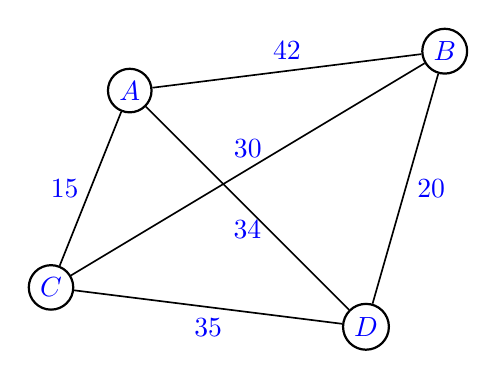
\begin{tikzpicture}[
    vertex/.style={
        circle, 
        draw=black, 
        thick,  
        inner sep=2pt, 
        font=\bfseries, 
        text=blue
    },
    weight/.style={
        font=\bfseries, 
        text=blue,
        inner sep=4pt 
    },
    edge/.style={
        semithick
    }
]
    \foreach \name/\x/\y in {
        A/1/2.5,
        B/5/3,
        C/0/0,
        D/4/-0.5%
    } {
        \node[vertex] (\name) at (\x, \y) {$\name$};
    }
    \foreach \u/\v/\w/\pos in {
        A/C/15/left,
        A/B/42/above,
        C/B/30/above,
        A/D/34/below,
        B/D/20/right,
        C/D/35/below%
    } {
        \draw[edge] (\u) -- node[weight, \pos] {$\w$} (\v);
    }

\end{tikzpicture}}
	\par\shortans[oly]{$99$}
	\loigiai{
		Không mất tính tổng quát, giả sử đoàn xuất phát từ địa điểm $A$. \\
		Để đi qua tất cả các địa điểm và quay về $A$, có các chu trình sau: 
\begin{itemize}
\item $A\to C\to B\to D\to A$: thời gian $15+34+20+30=99$. 
\item $A\to C\to D\to B\to A$: thời gian $15+35+20+42=112$. 
\item $A\to B\to C\to D\to A$: thời gian $42+34+35+30=141$. 
\item $A\to B\to D\to C\to A$: thời gian $42+20+35+15=112$. 
\item $A\to D\to C\to B\to A$: thời gian $30+35+34+42=141$. 
\item $A\to D\to B\to C\to A$: thời gian $30+20+34+15=99$. 
\end{itemize}
		Vậy tổng thời gian di chuyển nhỏ nhất là $99$.
	}
\end{ex}

\begin{ex}%[2D4H3-3]
	Trên mặt phẳng tọa độ $Oxy$, vẽ nửa đường tròn tâm $O$, bán kính $r=2$ nằm phía trên trục $Ox$. Gọi $D$ là hình phẳng giới hạn bởi nửa đường tròn, trục $Ox$ và đường thẳng $x=1$. Tính thể tích khối tròn xoay được tạo thành khi quay $D$ quanh trục $Ox$ ({\it kết quả làm tròn đến chữ số hàng phần chục}).
	\par\shortans[oly]{$28{,}3$}
	\loigiai{
		\begin{center}
		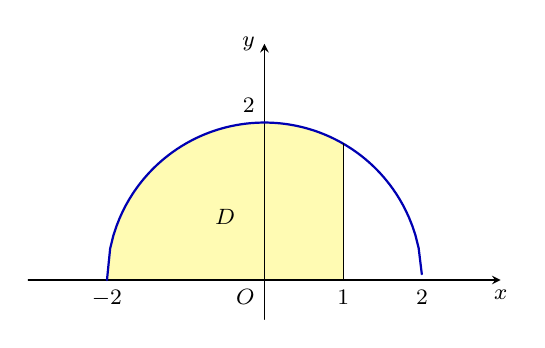
\begin{tikzpicture}[scale=1, font=\footnotesize, line join=round, line cap=round, >=stealth, declare function={f(\x)=sqrt(4-(\x)^2);}]
\fill[yellow!30] (-2,0) -- plot[domain=-2:1, samples=100] (\x, {f(\x)}) -- (1,0) -- cycle;
			\draw[->] (-3,0) -- (3,0) node[below] {$x$};
			\draw[->] (0,-0.5) -- (0,3) node[left] {$y$};
			\node[below left] at (0,0) {$O$};			
			\draw[thick, blue!70!black, domain=-2:2, samples=100] plot(\x, {f(\x)});
			\draw (1,0) node[below] {$1$} -- (1, {f(1)});
			\node[below] at (-2,0) {$-2$};
			\node[below] at (2,0) {$2$};
			\node[above left] at (0,2) {$2$};
			\node at (-0.5, 0.8) {$D$};
		\end{tikzpicture}
		\end{center}
		Phương trình đường tròn tâm $O$, bán kính $r=2$ là $x^2+y^2=4$. \\
		Nửa đường tròn nằm phía trên trục $Ox$ có phương trình $y=\sqrt{4-x^2}$. \\
		Hình phẳng $D$ được giới hạn bởi $y=\sqrt{4-x^2}$, $y=0$, $x=-2$, $x=1$ nên thể tích khối tròn xoay là
		$$V=\pi\displaystyle\int \limits_{-2}^1\left(\sqrt{4-x^2}\right)^2\,\mathrm{d}x=\pi\displaystyle\int \limits_{-2}^1(4-x^2)\,\mathrm{d}x=9\pi\approx28{,}3.$$
	}
\end{ex}

\begin{ex}%[2D5H2-3]
	Bạn Vân tham gia một cuộc thi về khoa học xã hội. Bộ câu hỏi của cuộc thi gồm $10$ câu hỏi lịch sử và $15$ câu hỏi địa lí. Xác suất Vân trả lời đúng một câu hỏi lịch sử là $0{,}6$ và một câu hỏi địa lí là $0{,}8$. Vân chọn ngẫu nhiên $1$ câu hỏi trong bộ câu hỏi. Biết rằng Vân trả lời đúng câu hỏi đó, tính xác suất để đó là câu hỏi lịch sử ({\it kết quả làm tròn đến hàng phần trăm}).
	\par\shortans[oly]{$0{,}33$}
	\loigiai{
		Tổng số câu hỏi là $25$ câu.\\
 Gọi \begin{itemize}
\item  $A$ là biến cố \lq\lq câu hỏi được chọn là câu hỏi lịch sử\rq\rq, ta có $\mathrm{P}(A)=\dfrac{10}{25}=0{,}4$. 
\item $\overline{A}$ là biến cố \lq\lq câu hỏi được chọn là câu hỏi địa lí\rq\rq, ta có $\mathrm{P}\left(\overline{A}\right)=\dfrac{15}{25}=0{,}6$. 
\item  $B$ là biến cố \lq\lq Vân trả lời đúng câu hỏi\rq\rq. Theo đề bài, $\mathrm{P}(B|A)=0{,}6$ và $\mathrm{P}\left(B|\overline{A}\right)=0{,}8$. 
\end{itemize}
		Áp dụng công thức Bayes, xác suất để câu hỏi đó là câu hỏi lịch sử khi biết Vân đã trả lời đúng là
		$$\mathrm{P}(A|B)=\dfrac{\mathrm{P}(A)\cdot \mathrm{P}(B|A)}{\mathrm{P}(A)\cdot \mathrm{P}(B|A)+\mathrm{P}\left(\overline{A}\right)\cdot \mathrm{P}\left(B|\overline{A}\right)}=\dfrac{0{,}4\cdot 0{,}6}{0{,}4\cdot 0{,}6+0{,}6\cdot 0{,}8}=\dfrac{0{,}24}{0{,}24+0{,}48}=\dfrac{0{,}24}{0{,}72}=\dfrac{1}{3}\approx0{,}33.$$
	}
\end{ex}

\begin{ex}%[2H2H1-4]
	Khi chuyển động trong không gian, máy bay luôn chịu tác động của $4$ lực chính: lực đẩy của động cơ, lực cản của không khí, trọng lực và lực nâng khí động học. Lực cản của không khí ngược hướng với lực đẩy của động cơ và có độ lớn tỉ lệ thuận với bình phương vận tốc máy bay. Một chiếc máy bay tăng vận tốc từ $900$ lên $920$, trong quá trình tăng tốc máy bay giữ nguyên hướng bay. Lực cản của không khí khi máy bay đạt vận tốc $900$ và $920$ lần lượt biểu diễn bởi hai véc tơ $\overrightarrow{F}_1$ và $\overrightarrow{F}_2$ với $\overrightarrow{F}_1=k\overrightarrow{F}_2$ ($k\in \mathbb{R};k>0$). Tính giá trị của $k$ ({\it kết quả làm tròn đến hàng phần trăm}).
\begin{center}
		\definecolor{deepskyblue}{rgb}{0.0, 0.75, 1.0}		
		\begin{tikzpicture}
			\clip (-4.5,-2.5) rectangle (4.5,2.5);
			\fill[bottom color=white,top color=deepskyblue!90, middle color=white] (-4.5,-2.5) rectangle (4.5,2.5);
			\begin{pgfinterruptboundingbox}
				
				%Đuôi máy bay
				\def\D{  (-2,-.45)--(-2.36,.24)--(-2.2,.3)--(-1.35,-.25)--cycle
					;}
				\draw \D;
				\fill[brown!40!] \D;
				
				%Quạt máy bay
				\def\Q{  (.15,-.1)
					..controls +(-140:0.1) and +(140:0.1) .. (.2,-.35)--(.8,-.17)--(.7,.07)--cycle
					
					;}
				\draw \Q;
				\draw[xshift=.5cm] \Q;
				\fill[brown!40!,xshift=.5cm] \Q;
				%---------elip2
				\draw[rotate=-70,xshift=-.23cm,yshift=1.27cm] (.7,-.1) ellipse (.12cm and .07cm);
				
				%Thân máy bay
				\def\T{  (-2.1,-.5)
					..controls +(40:0) and +(-170:0.7) .. (2,.74)
					..controls +(-40:0) and +(170:0.3) .. (2.55,.7)
					..controls +(-150:0) and +(30:.65) .. (2.1,.3)
					..controls +(-150:0) and +(-18:1.25) .. (-2.1,-.6)
					..controls +(90:0) and +(-90:0) .. (-2.1,-.51)
					-- (-2.5,-.52)--cycle;
				}
				\draw \T;
				\fill[brown!70!] \T;
				%Cánh máy bay
				\def\C{  (.5,.05)
					..controls +(170:0) and +(-10:0) .. (-1.48,.12)
					..controls +(-80:0) and +(170:0.02) .. (-1.65,.3)
					..controls +(180:0) and +(0:0) .. (-1.77,.3)
					..controls +(-80:0) and +(110:0) .. (-1.64,.12)
					..controls +(-35:0) and +(145:0) .. (-.2,-.17)
					--cycle
					;}
				\draw \C;
				\fill[brown!40!] \C;
				%Quạt sau
				\fill[brown!40!] \Q;
				%---------------Véc-tơ
				\draw[->] (.2,0)--(.2,-1.5)node[right] {Trọng lực};
				\draw[->,color=black] (.2,0)--(.2,1.5) node[right] {Lực nâng};
				\draw[->] (.2,-.05)--(2.9,0.8) node[above] {Lực đẩy};
				\draw[->] (.2,-.05)--(-2.9,-1.05) node[below,pos=0.9] {Lực cản không khí};
				%----elip 1
				\draw[rotate=-70,xshift=-.4cm,yshift=.8cm] (.7,-.1) ellipse (.12cm and .07cm);
				%Ô cửa
				\draw (2.18,0.73)--(2.5,0.7)--(2.14,0.58)--cycle;
				\fill[brown!40!](2.18,0.73)--(2.51,0.71)--(2.14,0.57)--cycle;
				
			\end{pgfinterruptboundingbox}
		\end{tikzpicture}		
	\end{center}
	\par\shortans[oly]{$0{,}96$}
	\loigiai{
		Vì máy bay giữ nguyên hướng bay nên hai véc tơ lực cản $\overrightarrow{F}_1$ và $\overrightarrow{F}_2$ cùng hướng, do đó $\overrightarrow{F}_1=k\overrightarrow{F}_2$ với $k>0$. \\
		Gọi $v_1,v_2$ lần lượt là vận tốc của máy bay. Ta có $v_1=900$, $v_2=920$. \\
		Vì độ lớn lực cản tỉ lệ thuận với bình phương vận tốc nên		$$k=\dfrac{\left|\overrightarrow{F}_1\right|}{\left|\overrightarrow{F}_2\right|}=\dfrac{v_1^2}{v_2^2}=\dfrac{900^2}{920^2}\approx0{,}96.$$
	}
\end{ex}

\begin{ex}%[2H2H2-6]
	Trong không gian $Oxyz$, một thiết bị phát sóng wifi đặt tại vị trí $A(3;1;1)$. Vùng phủ sóng tốt nhất của thiết bị có bán kính bằng $11$ (m). Hỏi số giá trị nguyên của tham số $m$ để một người sử dụng điện thoại tại điểm $E(-3;8;m)$ có thể bắt được tín hiệu wifi tốt nhất của thiết bị nói trên.
	\par\shortans[oly]{$13$}
	\loigiai{
	Để điện thoại tại $E(-3;8;m)$ bắt được tín hiệu tốt nhất thì khoảng cách $AE\le R$. \\
		Ta có $AE=\sqrt{(-3-3)^2+(8-1)^2+(m-1)^2}=\sqrt{36+49+(m-1)^2}=\sqrt{85+(m-1)^2}$. \\
		Yêu cầu bài toán tương đương với 
\begin{eqnarray*}
\sqrt{85+(m-1)^2}\le 11&\Leftrightarrow &85+(m-1)^2\le 121\\&\Leftrightarrow &(m-1)^2\le 36\\&\Leftrightarrow &-6\le m-1\le 6\\&\Leftrightarrow &-5\le m\le 7.
\end{eqnarray*} 
Vì $m\in \mathbb{Z}$ nên $m\in \{-5;-4;-3;\dots;7\}$. \\
Số giá trị nguyên của $m$ thỏa mãn là $7-(-5)+1=13$ (giá trị).
	}
\end{ex}

\begin{ex}%[2D1H3-6]
	Một chất điểm chuyển động có phương trình chuyển động là $s=-t^3+6t^2+17t$ với $t$ (s) là khoảng thời gian tính từ lúc vật bắt đầu chuyển động và $s$ (m) là quãng đường vật đi được trong khoảng thời gian đó. Trong khoảng thời gian $8$ giây đầu tiên, vận tốc $v$ (m/s) của chất điểm đạt giá trị lớn nhất bằng bao nhiêu?
	\par\shortans[oly]{$29$}
	\loigiai{
		Vận tốc của chất điểm là  $v(t)=s'(t)=-3t^2+12t+17$. \\
		Ta đi tìm giá trị lớn nhất của hàm số $v(t)$ trên đoạn $[0;8]$. \\
	Ta có $v'(t)=-6t+12$ và  $v'(t)=0\Leftrightarrow t=2\in [0;8]$. \\
Ta tính được $v(0)=17$, $v(2)=29$, $v(8)=-79$. \\
Vậy vận tốc lớn nhất trong khoảng $8$ giây đầu tiên là $29$ m/s (đạt được tại $t=2$ s).
	}
\end{ex}

\Closesolutionfile{ans}
\indapan{4}{ans/De-TB-Yeu-So-19}
